% This is LLNCS.DEM the demonstration file of
% the LaTeX macro package from Springer-Verlag
% for Lecture Notes in Computer Science,
% version 2.4 for LaTeX2e as of 16. April 2010
%
\documentclass{llncs}
%
\usepackage{makeidx}  % allows for indexgeneration
\usepackage{graphicx}
%
\begin{document}
%
\frontmatter          % for the preliminaries
%
\pagestyle{headings}  % switches on printing of running heads
\addtocmark{Hamiltonian Mechanics} % additional mark in the TOC
%
%\chapter*{Preface}


%
\mainmatter              % start of the contributions
%
\title{Optimized declarative transformation\\First Eclipse QVTc results}
%
\titlerunning{First Eclipse QVTc results}  % abbreviated title (for running head)
%                                     also used for the TOC unless
%                                     \toctitle is used
%
\author{Edward D. Willink\inst{1}}
%
\authorrunning{Edward D. Willink} % abbreviated author list (for running head)
%
%%%% list of authors for the TOC (use if author list has to be modified)
\tocauthor{Edward D. Willink}
%
%\institute{Willink Transformations Ltd., Reading, UK,\\
%\email{ed_at_willink.me.uk},}
\institute{Willink Transformations Ltd., Reading, UK,\\
\email{ed/at/willink.me.uk},
}

\maketitle              % typeset the title of the contribution

\begin{abstract}
It is over ten years since the first OMG QVT FAS\footnote{Object Management Group Query/View/Transformation Final Adopted Specification.} was made available with the aspiration to standardize the fledgling model transformation community. Since then two serious implementations of the operational QVTo language have been made available, but no implementations of the core QVTc language, and only rather preliminary implementations of the QVTr language. No significant optimization of these (or other transformation) languages has been performed. In this paper we present the first results of the new Eclipse QVTc implementation demonstrating scalability and major speedups through the use of metamodel-driven scheduling and direct Java code generation.
\keywords{optimization, declarative transformation, scheduling, code generation, QVTc}
\end{abstract}
%

\section{Introduction}

The OMG QVT specification~\cite{QVT-1.3-Beta} was planned as the standard solution to model transformation problems. The Request for Proposals in 2002 stimulated 8 responses that eventually coalesced into a revised merged submission in 2005 for three different languages.

The QVTo language provides an imperative style of transformation. It stimulated two useful implementations, SmartQVT and Eclipse QVTo. %Only Eclipse QVTo is still maintained.

The QVTr language provides a rich declarative style of transformation. It also stimulated two implementations. ModelMorf never progressed beyond beta releases. 
%It is no longer available.
Medini QVT had disappointing performance and is not maintained.

The QVTc language provides a much simpler declarative capability that was intended to provide a common core for the other languages. There has never been a QVTc implementation since the Compuware prototype was not updated to track the evolution of the merged QVT submission.

The Eclipse QVTd project~\cite{Eclipse-QVTd} extended and enhanced the Eclipse OCL~\cite{Eclipse-OCL} framework to provide QVTc and QVTr editors, but until now provided no execution capability. This paper describes two aspects of the architecture that promises a high performance remedy for this deficiency. In Section~\ref{Efficiency} we review the efficiency hazards that are addressed in Section~\ref{Architecture}. Section~\ref{Scheduling} describes the derivation of an efficient declarative schedule and Section~\ref{Results} presents preliminary results demonstrating some scalability and code generation speed-ups. Section~\ref{Related Work} summarizes some related work and Section~\ref{Conclusions} concludes.

\section{Efficiency}\label{Efficiency}

The execution time of each algorithm in a computer program is `obviously' the product of many factors: \((W.N.R.L.C)^A\)
\begin{itemize}
\item W - the Workload - the number of data elements to be processed
\item N - the Necessary computations per data element
\item R - the memory Representation access overhead
\item L - the programming Language overhead
\item C - the Control overhead
\item A - the Algorithmic overhead
\end{itemize}

We cannot optimize N or W since they represent the Necessary Work.

We have limited choice in regard to L since use of a more efficient Language than Java may incur tooling, portability or cultural difficulties. We have similarly limited choice in Representation since there may be few frameworks to choose from. We should however be aware that Java may cost a factor of two or three and that unthinking use of EMF~\cite{Eclipse-EMF} may incur a factor of ten (Figure~\ref{fig:Families2Persons}).

The Control overhead is influenced a bit by programming style, but mostly by the tooling approach, thus an interpreted form of execution may easily incur a ten-fold overhead when compared to a code generated one.

The above costs are all proportionate. Algorithmic cost is however exponential, normally with a unit exponent, but a poor algorithm may involve quadratic or worse costs. It is therefore recognized that the best way to improve performance is to discover a better algorithm, or, more practically, to replace a stupid algorithm that performs repeated or unnecessary work.

For a  model transformation using an imperative transformation language, the programmer specifies the algorithms (mappings) and the control structures that invoke them (mapping calls). We hope that the programmer selects good algorithms and that the tooling for the transformation language implements them without disproportionate overheads so that the overall execution incurs only proportionate costs relative to the given program's Necessary Work.

When we use a declarative model transformation, the control structures are no longer defined by the programmer. A control strategy must be discovered by the transformation tooling. This has the potential to give improved performance since a better control strategy may be discovered than that programmed imperatively. On the other hand, inferior declarative transformation tooling may incur Control overheads that result in disproportionate Algorithmic overheads.

In this paper we outline approaches that avoid Algorithmic overheads and since we use code generation to Java, we compound a perhaps five-fold reduction in Representation access and a perhaps five-fold reduction in Control overhead when compared to an interpreted execution using dynamic EMF.

\section{Architecture}\label{Architecture}

The Eclipse QVTd architecture for QVTr and QVTc `solves' the problem of  implementing a triple language specification by introducing Yet Another Three QVT Languages\cite{ya3qvt} : QVTu, QVTm and QVTi. Subsequent scheduler development has introduced two more languages QVTp and QVTs for use in the transformation chain shown in Figure \ref{fig:architecture}.

\begin{figure}[h]
	\centering
	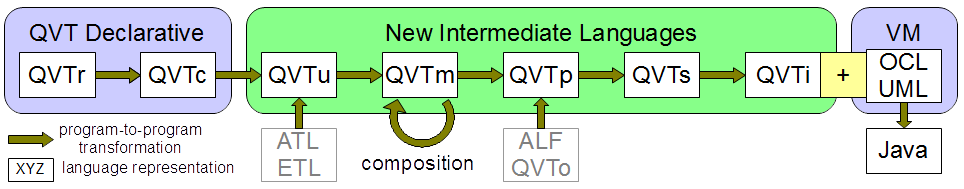
\includegraphics[width=1.0\textwidth]{QVThorizontalAlphabet.png}
	\caption{Progressive transformation approach for Declarative QVT.}
	\label{fig:architecture}
\end{figure}

\paragraph{QVTr2QVTc} implements the RelToCore transformation only partially defined by the QVT specification. This is still a work in progress.

\paragraph{QVTc2QVTu} exploits the user's chosen direction to form a Unidirectional transformation without the bloat for the unwanted directions.

\paragraph{QVTu2QVTm} normalizes and flattens to form a Minimal transformation free from the complexities of mapping refinement and composition.

\paragraph{QVTm2QVTp} Partitions mappings into micro-mappings that are free from deadlock hazards.

\paragraph{}The foregoing representations use increasingly restricted semantic subsets of the QVTc language.

\paragraph{QVTp2QVTs} creates a graphical representation suitable for dependency analysis enabling an efficient Schedule to be planned.

\paragraph{QVTs2QVTi} serializes the graphical representation and schedule into an Imperative extension and variation of the QVTc language. This can be executed directly by the QVTi interpreter that extends the OCL Virtual Machine. Alternatively an extended form of the OCL code generator may be used to produce Java code directly. This bypasses many of the overheads of interpreted execution or dynamic EMF. The generated code comprises one outer class per-transformation. Each mapping is realized as either a nested class or a function depending on whether state is needed to handle repeated or premature execution.

\section{Scheduling}\label{Scheduling}

\subsection{Naive Schedule}

A declarative transformation can always execute using the naive polling schedule
\begin{itemize}
\item Retry loop - loop until all work done
\item ~~Mapping loop - loop over all possible mappings 
\item ~~~~Object loops - multi-dimensional loop for all object/argument pairings
\item ~~~~~~Compatibility guard - if object/argument pairings are type compatible
\item ~~~~~~Repetition guard - if this is not a repeated execution
\item ~~~~~~Validity guard - if all input objects are ready
\item ~~~~~~Execute mapping for given object/argument pairings
\item ~~~~~~Create a memento of the successful execution
\end{itemize}

This is hideously inefficient with speculative executions wrapped in at least three loops, guards and mementos when compared to a simple linear `loop' nest.

The key functionality of a declarative model transformation comprises a suite of OCL expressions that relates output elements and their properties to input elements and their properties using metamodels to define the type system of the elements and properties. The suite of OCL expressions is structured as mappings that provide convenient re-usable modules of control.

\subsection{Metamodel-driven planning, micro-mappings}

The metamodel type system enables producer/consumer relationships to be established between mappings. These relationships can be used by an intelligent `Mapping loop' to avoid many of the retries that result from careless attempted execution of consumers before producers. Similarly, considering only type compatible objects in the `Object loops' eliminates another major naivety. 

Analysis of the types alone is of limited value, since each type may have many properties. Each property assignment must be analyzed separately to avoid deadlock hazards. For instance, an attempt to assign both forward and backward references of a circular linked list at once deadlocks somewhere round the loop. Therefore a declarative mapping that appears to assign all properties at once, must be broken up into smaller micro-mappings to avoid a deadlock hazard. In practice fewer than 10\% of mappings appear to need partitioning into micro-mappings, and once a valid schedule has been established, some of these can be merged.

The `Object loops' can be very inefficient even when restricted to type compatible objects, since the number of permutations grows exponentially with the number of inputs. For genuinely independent inputs this cost is fundamental and the only solution is for the programmer to provide a better algorithm that exposes a dependence. In practice many objects have a very strong relationship such as between a parent and a child object. From the parent there may be many child candidates, but from the child there is only zero or one parent object. We therefore replace the parent as an externally searched input by an internally derived computation. This reduces the order of the input permutation. In practice between 90\% and 100\% of micro-mappings can be simplified to only one input.

A micro-mapping either executes successfully updating its outputs, or fails completely updating nothing until a later successful re-execution. Failure occurs whenever the computation prematurely navigates from one object to another. We therefore want to identify as many of the objects that a micro-mapping may access in order to provide a static schedule in which consumed objects are produced first. 

\subsection{Intra-micro-mapping scheduling}

Of course at compile-time we have no instances, just types which only give us limited producer-consumer precision. However the constraints in a declarative transformation define patterns that enable us to relate multiple types. Our QVTp2QVTs analysis therefore starts with a transliteration from partitioned QVTc as shown in Figure~\ref{fig:ClassToTable.qvtp} to graphical form as shown in Figure~\ref{fig:ClassToTable.qvts}

\begin{figure}[h]
	\centering
	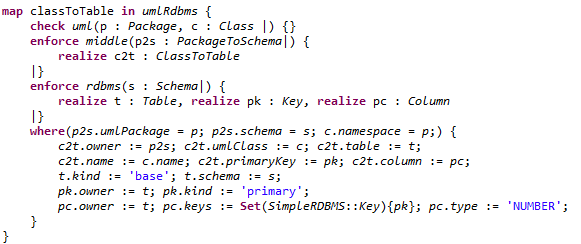
\includegraphics[width=1.0\textwidth]{ClassToTable-qvtp.png}
	\caption{Class-to-Table mapping in partitioned QVTc (QVTp).}
	\label{fig:ClassToTable.qvtp}
\end{figure}

\begin{figure}[h]
	\centering
	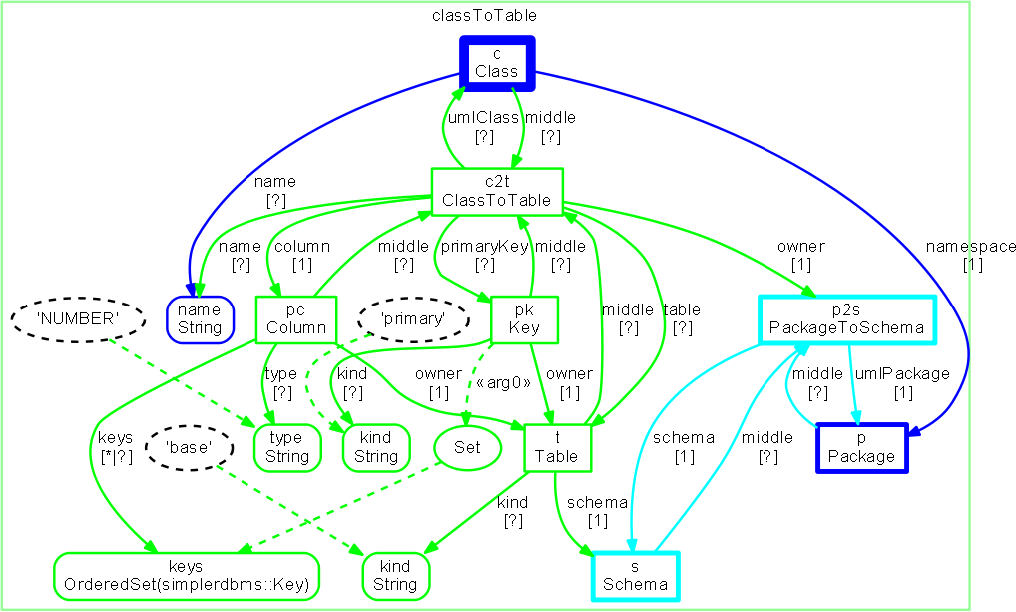
\includegraphics[width=1.0\textwidth]{ClassToTable-qvts.png}
	\caption{Class-to-Table mapping in graphical form (QVTs).}
	\label{fig:ClassToTable.qvts}
\end{figure}

The example is taken from the ubiquitous UML to RDBMS example and shows the mapping from a Class (child of a Package) to a Table (child of a Schema) and since we are using QVTc, the intermediate trace is programmed explicitly as a ClassToTable. The textual representation in  Figure~\ref{fig:ClassToTable.qvtp} shows a two input (p, c), two output (p2s,  s) interface and four creations (c2t, t, pk, pc). The parentheses of the where clause show three pattern matching constraints. The braces of the where clause show thirteen assignments.

The graphical form is inspired in part by Henshin~\cite{Henshin} but with additional colors. Black indicates what is constant at compile-time. Blue shows what is loaded from input models. Green indicates what is created. Additionally Cyan identifies what is consumed after it is produced elsewhere.

Solid edges show something-to-one unidirectional navigation paths between rectangular class instances and their rounded-rectangular attributes. Nodes are annotated with instance name and type, edges with property name and multiplicity. Dashed edges and ellipses show computations rather than navigations.

Bidirectional navigations are shown as pairs of unidirectional edges, but only something-to-one navigations are shown. Consequently any navigation edge may be traversed in its forward direction to the precisely one object that matches the pattern element. Following all the paths in this way identifies that all navigable objects can be reached unambiguously from the c:Class input. This is drawn with a very thick boundary to emphasize its importance. What appeared to be a 4-input mapping in textual form is actually a 1-input mapping, so what appeared to challenge the scheduler with a 4-dimensional search is realizable with a 1-dimensional loop.

The graphical form therefore clearly shows, in blue, that we need to match a c:Class in the loaded input model that has a Package at c.namespace and a String at c.name. Additionally the cyan shows that execution is not possible until p.middle provides p2s and p2s.schema provides s. Once these are all available, the many objects and relationships shown in green can be produced. We therefore have a very simple dependency rule; every cyan node or edge must be produced by a corresponding green node or edge in another micro-mapping.

\subsection{Inter-micro-mapping scheduling}

In practice it is not quite so simple because we must account for multiple producers and derived types. But in principle we can just join all the micro-mappings up with dependencies to derive the schedule as shown in Figure~\ref{fig:UML2RDBMS.qvts}\footnote{One rectangle, two ellipses and associated lines have been removed so that the nodes and edges are discernible; the lettering is not relevant.}.

\begin{figure}[h]
	\centering
	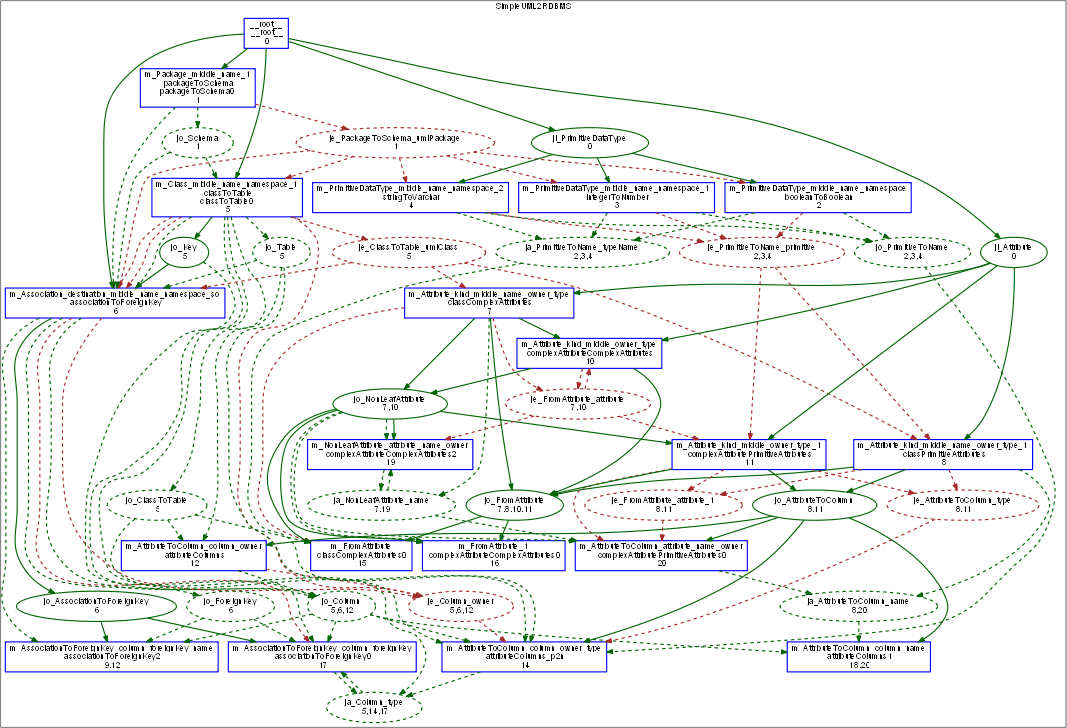
\includegraphics[width=1.0\textwidth]{UML2RDBMS-qvts.png}
	\caption{UML2RDBMS schedule in graphical form (QVTs).}
	\label{fig:UML2RDBMS.qvts}
\end{figure}

At the top, the root pseudo mapping is a producer of input model elements, triaged as allInstances of interesting types. These are consumed by the 19 rectangles one for each merged micro-mapping of the transformation.

Solid edges pass model elements to each consuming input. Simple connections are drawn directly. Multiple producers or multiple consumers are drawn through an intermediate ellipse which corresponds to a buffer that accumulates inputs from many producers and then makes them available to many consumers.

Further connections are shown using dashed edges and ellipses. These can easily be recomputed by the consumer and so no connection needs to be reified, however the schedule must ensure that the producer produces before the consumer consumes. Thus for the ClassToTable example, a Class is passed via a solid edge; the other three inputs are computed by navigation from the one input. These computations fail until the dashed dependencies have been satisfied.
%We can say that solid edges are pass-by-tangible-value whereas dashed edges are pass-by-existential-value. The dark green dashed edges are node-to-node dependencies.
%Brown dashed edges are edge-to-edge dependencies. Thus for ClassToTable dark green dashed edges ensure that the p2s and s exist, brown dashed edges ensure that they are interconnected.
The many (75\%) dashed elements shows a useful compile-time optimization.
% that eliminates parameters and intermediate buffers.

A sequential schedule is derived by allocating an integer slot index to each micro-mapping in turn such that all its predecessors have smaller indexes. In practice, a perfect static schedule can often be derived, but sometimes a recursion may introduce a cyclic dependency that can only be resolved at run-time. For this small proportion of micro-mappings additional run-time support is activated so that a failed speculative execution blocks according to the failure and retries only once the failure cause has been resolved. Few micro-mappings incur multiple failures and so in practice the retry overhead is less than 50\% and only where the data relationships exceed the compile-time analysis capability.

Three of the nineteen UML2RDBMS micro-mappings require two inputs. This incurs a quadratic tooling algorithm inefficiency that shows up when the performance is measured for input models containing associations. For just packages, classes and properties, the execution scales linearly with Workload. Examination of these three mappings reveals that there is a 1:N relationship between a primary and a secondary part of the mapping. Future work includes an optimization to treat the primary input as the one input and derive the secondary input using a local loop. This local loop can iterate only over matches, whereas the current external global loop iterates over many mismatches.

%This demonstrates how the combination of metamodel constraints and graph form exposition facilitate the identification of scheduling optimizations that alleviate bad algorithmic overheads.

\section{Results}\label{Results}

As just described, the performance of the QVTc variant of UML2RDBMS scales linearly when the input model contains just packages, classes and properties, but, pending further work, goes quadratic once associations are added.

In this section we plot the performance of the simple Familes2Persons transformation that involves a two-way guarded decision around a copy\footnote{Model overheads are reduced by Java code generated by an EMF genmodel.}. The plot demonstrates the scalability and the underlying tooling efficiency.\footnote{The plots use no averaging. Single point wobbles may be due to concurrent activity. Multiple point wobbles may be due to fortuitous cache alignment.}

\begin{figure}[h]
	\centering
	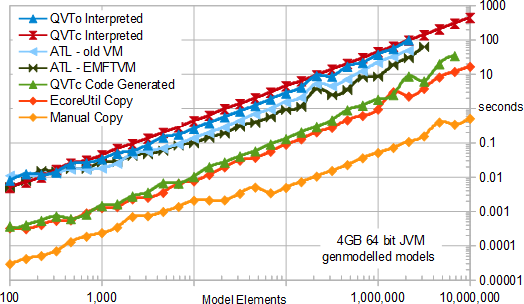
\includegraphics[width=1.0\textwidth]{Families2Persons.png}
	\caption{Performance of the simple Familes2Persons transformation.}
	\label{fig:Families2Persons}
\end{figure}

The top two lines of Figure \ref{fig:Families2Persons} show the performance of the new interpreted QVTc and contrasts it with the Eclipse QVTo. There is very little difference, except that QVTo has a much higher trace overhead and so fails to execute beyond 2,500,000 elements; an unexpected advantage of the explicit QVTc trace.

The two lines slightly below these show the old and new ATL VMs. Both fail to get close to 10,000,000 elements in the 4GB 64 bit VM.

The next two lines are about 30 times faster and contrast the new code generated QVTc with the standard EcoreUtil copy functionality. QVTc is currently about 20\% slower and just fails to reach 10,000,000 elements.

The final line is a manually coded implementation of the copy that bypasses the overheads of dynamic EMF in similar fashion to the code generated QVTc. For large numbers of model elements,
%\footnote{many model elements use many addresses, fewer elements use fewer addresses which may incur cache misses disproportionately}
this is about twenty times faster indicating that there is considerable scope for further improvement using the current approach. Using a non-EMF model representation can give further improvements and moving to C execution yet more.

%Failure of such a simple transformation at around 10,000,000 model elements in a 4 GB VM is disappointing. It suggests a 400 bytes per model element cost. Use of a modern 64 bit processor incurs an 8 byte cost for every thing, so 400 bytes is 50 things per model element. Each model element involves a String and a few pointers. For each model element, there is an input, an output and an intermediate object, pointers to them and also a surprisingly large HashMap node. Perhaps a 25\% saving is available with smarter implementation. Optimizing the representation to suit the transformation can save much more. An even larger saving may be made by trading off size for speed so that one, two or four byte values are used rather than eight bytes always.

\section{Related Work}\label{Related Work}

The idea of generalizing the concepts of a Java Virtual Machine to a Modeling Virtual Machine is attractive and has influenced ATL~\cite{Eclipse-ATL}. However while its original representation had small byte-code-like concepts, they were far from byte-sized. The newer EMFTVM  is therefore able to do significantly better~\cite{EMFTVM-performance}, but retains a transformation structure that supports transformation with OCL expressions as an afterthought. EMFTVM is 80\% slower than its EcoreUtil `optimum'. In contrast the OCL VM uses the OCL Abstract Syntax as its `byte-code' and supports extension to the QVTi AS so that all AS elements form part of a single executable element hierarchy. The performance reported in the previous section was 20\% slower than EcoreUtil but the `optimum' target for further work is ten times faster than EcoreUtil. 

Code generation has not been pursued by other transformation engines, perhaps because OCL code generation is not easy. Superficially there are similarities between OCL and Java and so a number of researchers have performed simple text template mapping~\cite{Wilke-CG}. This works sometimes, but fails to handle OCL in general. In contrast the Eclipse OCL Java code generator converts the OCL AS to an intermediate CG AS upon which a number of optimizations and rewrites are performed before Java code is emitted. The code generator supports all OCL constructs and its extensibility is demonstrated by its re-use for QVTi.

The Graph Transformation community has been very active in providing a rigorous foundation for graph mappings. Sadly the QVT specification ignored this important work, preferring instead to define the semantics of the QVTr transformation language using an incomplete exposition of a transformation of QVTr written in an untested QVTr to another language (QVTc) that has at best informal semantics. The utility and power of the graphical QVTs representation may begin to bridge the gap between these two communities. The coloring in QVTs is inspired by the use of colors to denote create/delete/no-change in endogenous transformations. The reification of the QVTc traceability element mirrors the evolution operators in UMLX~\cite{UMLX} for heterogeneous transformations.

Active Operations~\cite{Jouault-ActiveOperations} also reify mappings 
%at run-time
to persist the state necessary for incremental execution. Micro-mappings similarly support incremental execution, but their primary rationale is to be a deadlock-free unit of computation.

%\section{Future Work}

%Execution capability has been slow to appear in Eclipse QVTc and what is presented here is far from a complete capability.

%\subsection{Transformation modes}

%Currently there is only a transformation capability, that is an ability to convert input models to output models. The surrounding interfaces to exploit the capability to perform checks, updates or in-place transformation is missing. The support for incremental execution is incomplete.

%\subsection{Speed Optimization}

%The planned schedule and Java code generation give significant benefits, but they have yet to be optimized and many other areas for optimization have been identified.

%\subsection{Space Optimization}

%The size of the generated transformation can be improved, but is not perceived to be significant.

%The amount of memory required for input, intermediate and output model elements is disappointing, particularly on modern 64 bit machines. Only modest improvements are feasible while continuing to use EMF representations. More significant improvements should be possible by auto-generating a metamodel-specific proprietary representation. 

%\subsection{QVTr}

%As indicated in \ref{qvtr}, the QVTc implementation introduced here is a large part of a future QVTr implementation. (At the time of writing only collection-free QVTr transformations are usable.)

%\subsection{QVTo}

%Eclipse QVTo is currently independent of the QVTd developments. It is planned to migrate to exploit the code generation capabilities. (Defining QVTo semantics with a QVTo2QVTp transformation could allow scheduling to be exploited too.)

\section{Conclusions}\label{Conclusions}

We have introduced the first implementation of the QVTc specification.

We have introduced the first direct code generator for model transformations.

We have shown that the direct code generator gives a thirty fold speed-up.

We have shown how a graph presentation of metamodel and dependency analyses tames the naive inefficiencies of a declarative schedule.

We have reported first results and mentioned some future works. Many more optimizations to do, and of course, QVTr.
%that with a planned schedule declarative transformations do not have to be slower than imperative transformations.

%
% ---- Bibliography ----
%
% EMF EMTVM QVT eOCL GT DresdenOCLCG ActiveObjects ?IncQuery
\begin{thebibliography}{5}
\bibitem {Henshin}
Biermann, E., Ermel, C., Schmidt, J., Warning, A.:
Visual Modeling of Controlled EMF Model Transformation using HENSHIN
Proceedings of the Fourth International Workshop on Graph-Based Tools, GraBaTs 2010.

\bibitem{Eclipse-ATL}
Eclipse ATL Project.\\
\url{https://projects.eclipse.org/projects/modeling.mmt.atl}

\bibitem{Eclipse-EMF}
Eclipse EMF Project.\\
\url{https://projects.eclipse.org/projects/modeling.emf.emf}

\bibitem{Eclipse-OCL}
Eclipse OCL Project.\\
\url{https://projects.eclipse.org/projects/modeling.mdt.ocl}

\bibitem{Eclipse-QVTd}
Eclipse QVT Declarative Project.\\
\url{https://projects.eclipse.org/projects/modeling.mmt.qvtd}

\bibitem{EMFTVM-performance}
EMFTVM performance.\\
\url{https://wiki.eclipse.org/ATL/EMFTVM\#Performance}

\bibitem{Jouault-ActiveOperations}
Jouault, F., Beaudoux, O.:
On the Use of Active Operations for Incremental Bidirectional Evaluation of OCL
15th International Workshop on OCL and Textual Modeling, Ottawa, 2015

\bibitem {Wilke-CG}
Wilke, C.: Java Code Generation for Dresden OCL2 for Eclipse, February 19, 2009.
\url{http://claaswilke.de/publications/study/beleg.pdf}

\bibitem{UMLX}
Willink, E: UMLX : A Graphical Transformation Language for MDA
Model Driven Architecture: Foundations and Applications, MDAFA 2003, Twente, June 2003.
\url{http://eclipse.org/gmt/umlx/doc/MDAFA2003-4/MDAFA2003-4.pdf}

\bibitem {ya3qvt}
Willink, E.:
Yet Another Three QVT Languages.
ICMT 2013 (2013)

\bibitem{QVT-1.3-Beta}
OMG. Meta Object Facility (MOF) 2.0 Query/View/Transformation Specification, Version 1.3 Beta.
OMG Document Number: ptc/15-10-02, March 2016.
\end{thebibliography}
\end{document}
